\label{ch:implementation}

Besides the realization of EDA sensors results relatively simple when compared with the circuitry of other devices, its limited diffusion at present implies a series of issues that are required to be addressed. More specifically:

\begin{itemize}
    \item EDA wearables oriented to research purposes tend to be \textbf{particularly expensive} (and most of the time unaffordable for small research projects)
    \item Well-known devices implementing EDA-related features do not provide Application Programming Interfaces for developers and do not provide open-source solutions either
\end{itemize}

The following chapter describes the implementation of a \textbf{simple} and completely \textbf{open-source} wearable device, aimed at providing a low-cost framework for the Electrodermal Activity measurement in \textbf{experimental contexts}.

\section{BITalino Electrodermal Activity Sensor}\label{sec:bitalino}

The sensor unit employed is the purpose-built \textbf{Electrodermal Activity Sensor} by \textbf{BITalino}. This constitutes a single module aimed at composing, along with many others sold by the company, the \textbf{BITalino (r)evolution Board Kit} \cite{bitalino-general}, an all-in-one device implementing a custom firmware for the collection and aggregation of data retrieved from bio-signals. Besides all the features implemented by these boards result interesting in research contexts, the main drawbacks are related to the \textbf{lack of mobility} that the device would cause, which is a primary concern within the bounds of fall detection systems.

Moreover, during the recent years the BITalino EDA module has been employed in a multitude of scientific publications which, overall, have proven that the device allows to reach optimal results in terms of cost-effective Electrodermal Activity analysis.

A \textbf{single EDA module} was purchased for a 25,00 € (Tax Excluded) price and a minimal \textbf{Arduino-based firmware} was implemented in order to retrieve measurements from the individual unit without having to rely on third-party solutions.

\subsection{Description and Features}\label{subsec:bitalino-features}

The EDA sensor module consists of a breakout board whose dimensions correspond to 12mm x 27mm \cite{bitalino-general}. A complete list of informations regarding the configuration of the unit is reported in Table \ref{toc:bitalino-features} .

\begin{table}[H]
\centering
\begin{tabular}{ll}
    \hline
    Parameter               & Value \\
    \hline
    Current                 & DC \\
    Range                   & 0-30 $\mu S$ \\
    Consumption             & $\pm 0.1 mA$ \\
    Bandwidth               & 0 - 2.8 Hz \\
    Measurement             & continuous \\
    Input Voltage Range     & 1.8 - 5.5 V \\
    \hline
\end{tabular}
\caption{Characteristics of the BITalino EDA sensor unit}
\label{toc:bitalino-features}
\end{table}

Furthermore, the device is sold in the three following configurations, according to the requirements of the customers: 
\begin{itemize}
    \item \textbf{Self-assemble}
    \item \textbf{Self-assemble} with \textbf{UC-E6 connectors}
    \item \textbf{Assembled}
\end{itemize}

\vspace{3mm}

The first version consists of the breakout board only and requires manual soldering to obtain a complete configuration. The second one provides, instead, pre-installed UC-E6 connectors in order to facilitate the connection to a BITalino board by using apposite homonymous cables. The assembled version is, lastly, presented as a ready-made configuration that includes: 

\begin{itemize}
    \item Pre-soldered electrodes
    \item Pre-soldered UC-E6 cable
    \item A 3D printed ABS case containing the breakout board
\end{itemize}

% https://bitalino.com/storage/uploads/media/homeguide4-eda.pdf

\subsection{Modifications applied}\label{subsec:bitalno-modifications}

In order to exploit the convenience provided by the case and the pre-soldered electrodes, an \textbf{assembled unit} was acquired and subsequently \textbf{modified} in order to implement the connection with a third-party microcontroller. More specifically, the modification procedure consisted of the following steps: 

\begin{enumerate}
    \item Opening of the ABS case
    \item Desoldering the four UC-E6 connector cables from their respective pins on the breakout board
    \item Soldering a dupont cable on each one of the pins
    \item Widening the cable conduit of the ABS case in order to allow the passage of the previously soldered cables
    \item Closing back the ABS case
\end{enumerate}

The role of the pins provided by the breakout board is depicted by the diagram reported in figure \ref{fig:bitalino-pinmap}

\begin{figure}[h]
    \centering
    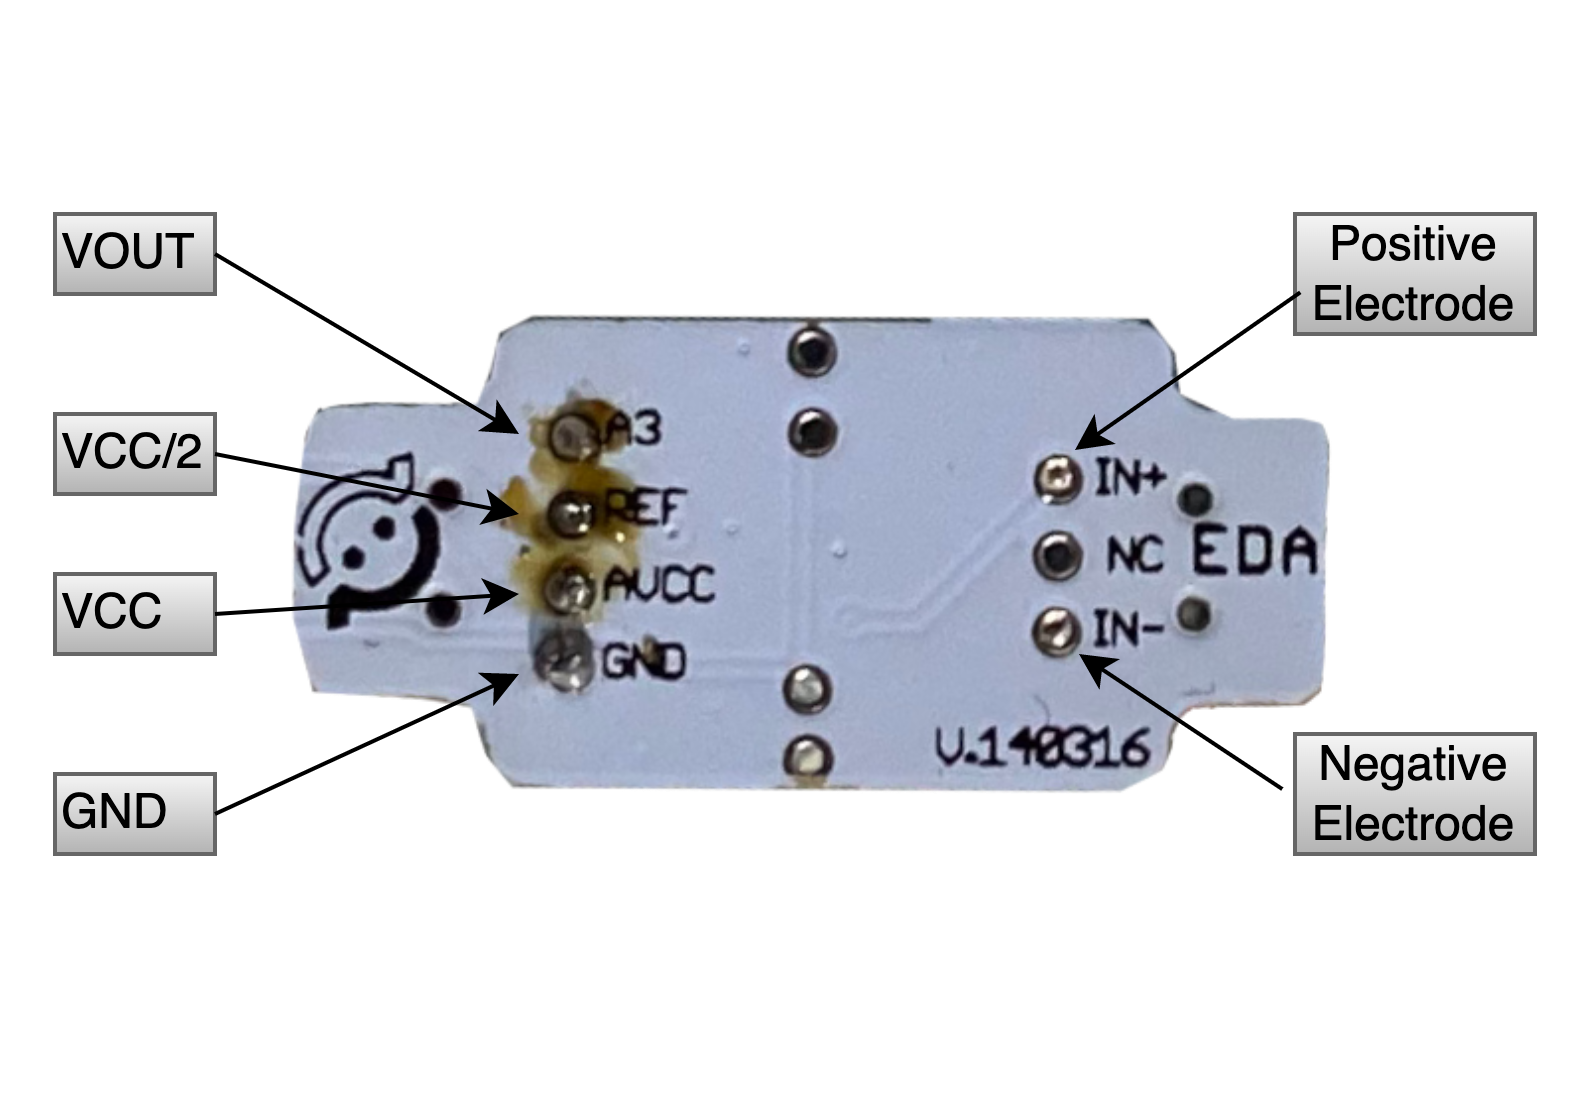
\includegraphics[width=10cm]{./images/bitalino.drawio.png}
    \caption{BITalino EDA sensor pin-map}
    \label{fig:bitalino-pinmap}
\end{figure}

\vspace{1cm}

More specifically, the function of each pin is reported in table \ref{toc:bitalino-pinmap-table}

\begin{table}[H]
\centering
\begin{tabular}{ll}
    \hline
    \textbf{Pin}            & \textbf{Application} \\
    \hline
    \texttt{IN+}            & Connection input for the positive electrode \\
    \texttt{IN-}            & Connection input for the negative electrode \\
    \texttt{A3}             & Analog output for the EDA signal reading \\
    \texttt{VCC/2}          & Midpoint voltage input, necessary for the microSiemens conversion \\
    \texttt{VCC}            & 3.3 V Voltage input \\
    \texttt{GND}            & Ground input \\
    \hline
\end{tabular}
\caption{Description of the BITalino EDA sensor pin-map}
\label{toc:bitalino-pinmap-table}
\end{table}

\vspace{1cm}

The result obtained after the aforementioned modifications were applied is reported in figure \ref{fig:full-sensor-configuration}. 

\begin{figure}
    \centering
    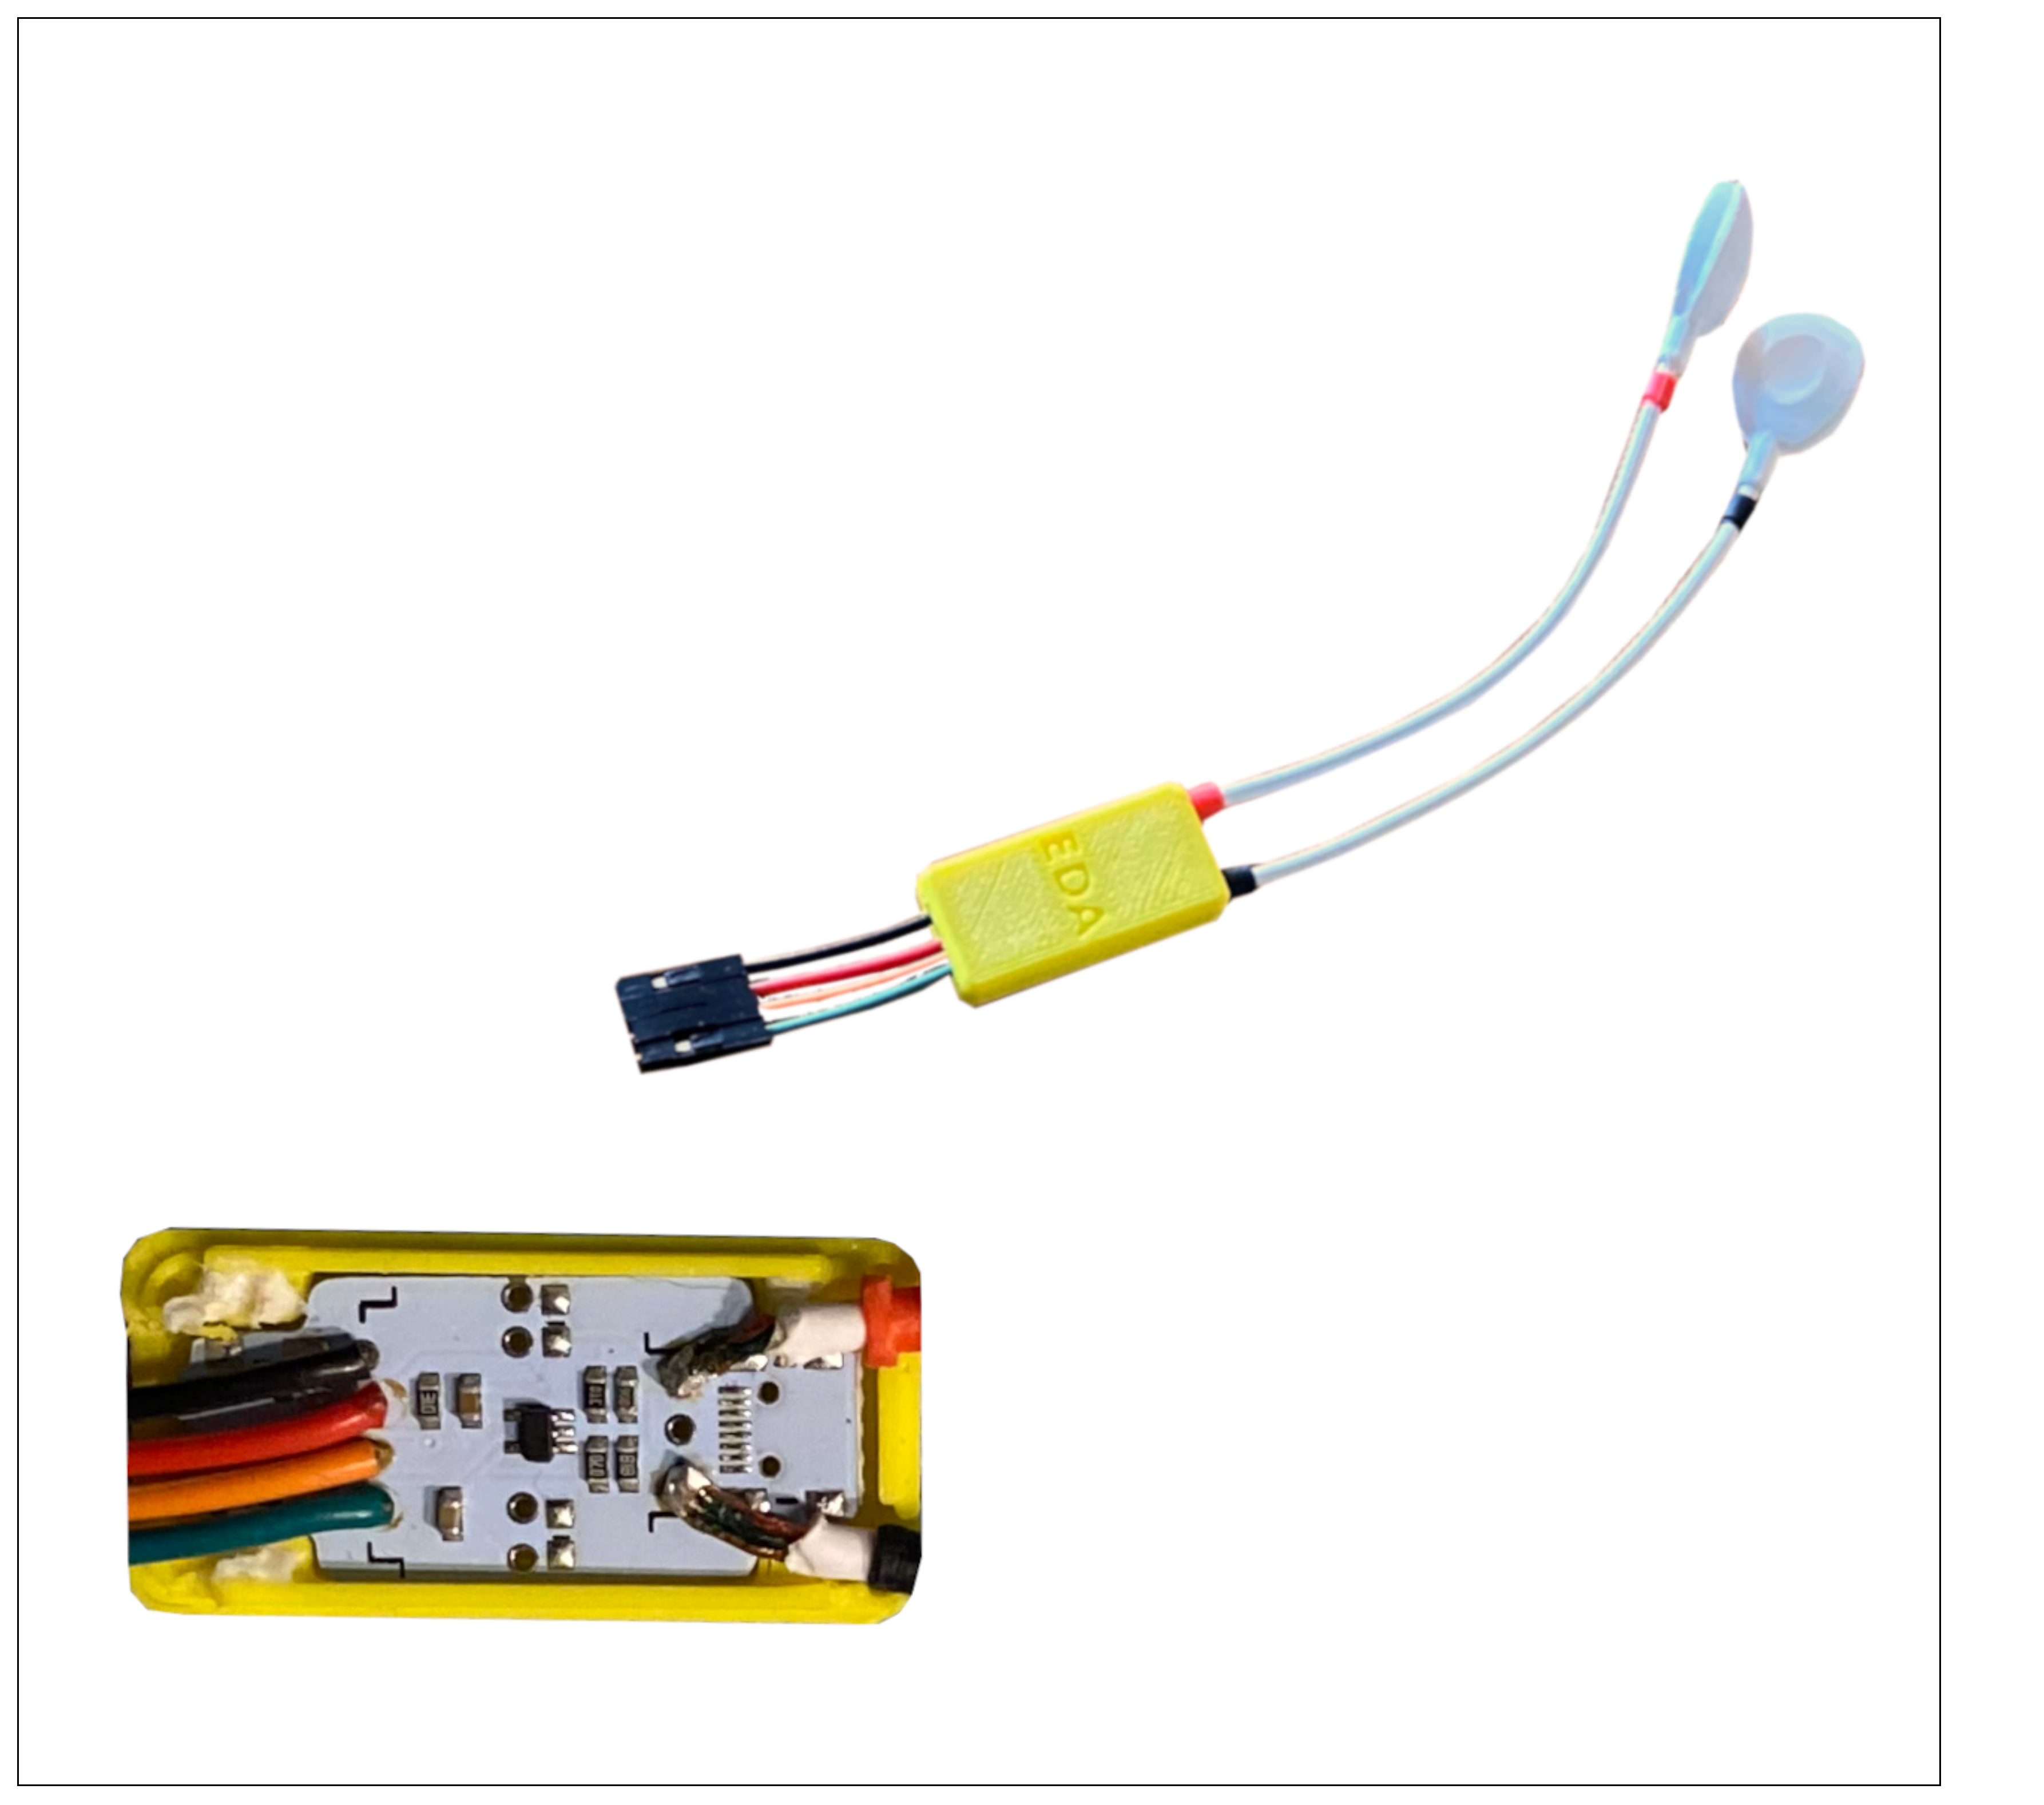
\includegraphics[width=10cm]{./images/full-sensor-view.drawio.png}
    \caption{End result after applying the modifications described}
    \label{fig:full-sensor-configuration}
\end{figure}

It is important to note the role of the \texttt{VCC/2} pin, which permits the flow of a so-called mid-point voltage through the circuit. This provides the necessary \textbf{stability} in order to compute the microSiemens value corresponding to signal measured basing on the output voltage obtained by the sensor \cite{bitalino-midpoint-voltage}. With the aim of providing a correct tension to the \texttt{VCC/2} pin, a voltage divider was implemented by employing two $100 k\Omega$ resistors according to the schematization reported in figure \ref{fig:voltage-divider-schema} 

\begin{figure}
    \centering
    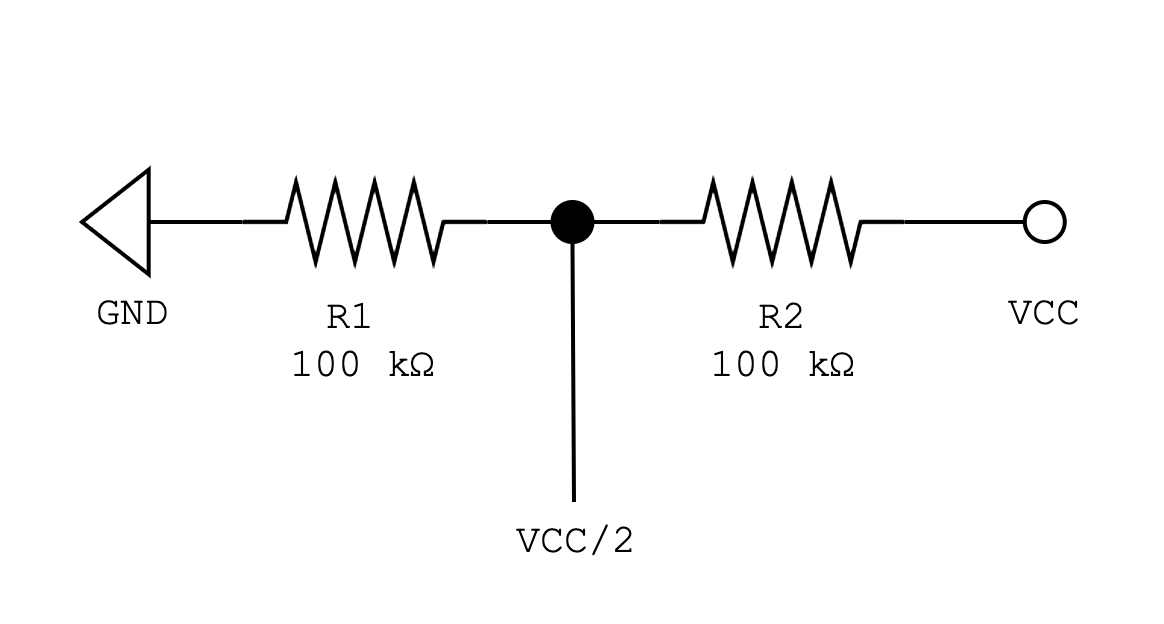
\includegraphics[width=11cm]{./images/midpoint-resistor.drawio.png}
    \caption{Mid-point resistor implemented for the \texttt{VCC/2} pin}
    \label{fig:voltage-divider-schema}
\end{figure}

\section{Developing a firmware based on the Arduino Framework}\label{sec:firmware}

After applying the necessary changes to the EDA sensor, a research was conducted in order to select an optimal microcontroller upon the following principles: 

\begin{itemize}
    \item Providing a cost-effective solution
    \item Dimensions geared towards high mobility contexts such as fall detection experimentations
    \item Ability to control the system remotely
    \item Limited battery consumption
\end{itemize}

\subsection{Hardware Employed}\label{sec:hardware-employed}

In accordance with the above-stated requirements, a unit based on the well-known \textbf{ESP8266} was employed. The latter consisted, more specifically, of the \textbf{D1 Mini by Wemos} board, which provides easy access to a multitude of functionalities maintaining limited dimensions.

\subsubsection{An overview of the ESP8266}\label{sec:esp8266}

% cite https://en.wikipedia.org/wiki/ESP8266

The ESP8266 consists of an inexpensive 32-bit microcontroller based on the L106 RISC microprocessor that is produced by Espressif Systems. It is widely known and employed in IoT contexts because of its limited dimensions and its native implementation of a full TCP/IP stack, allowing the development of networking-based applications without the requiring additional hardware \cite{esp8266}.

Furthermore, the unit exposes 17 GPIO pins and allows 










